% !Mode:: "TeX:UTF-8"
\chapter{研究背景}
\section{对抗攻击及对抗训练}
机器学习在人脸识别、语音识别、目标检测等应用领域已得到广泛普及,神经网络也广
泛部署在这些可能涉及用户隐私和安全的应用中,完成重要推断。然而研究表明,神经网络
对于来自人的恶意攻击脆弱而敏感\cite{DBLP:journals/corr/SzegedyZSBEGF13}。这种攻击通过在神经网络的输入中针对模型特点施加一
定扰动,使得模型预测产生较大偏差。对抗训练将经过特殊扰动的攻击性数据纳入训练数据
集,以使得机器学习模型对于外部攻击具有更高的稳定性(图\ref{fig:adv_train})。
\begin{figure}[htbp]
    \centering
    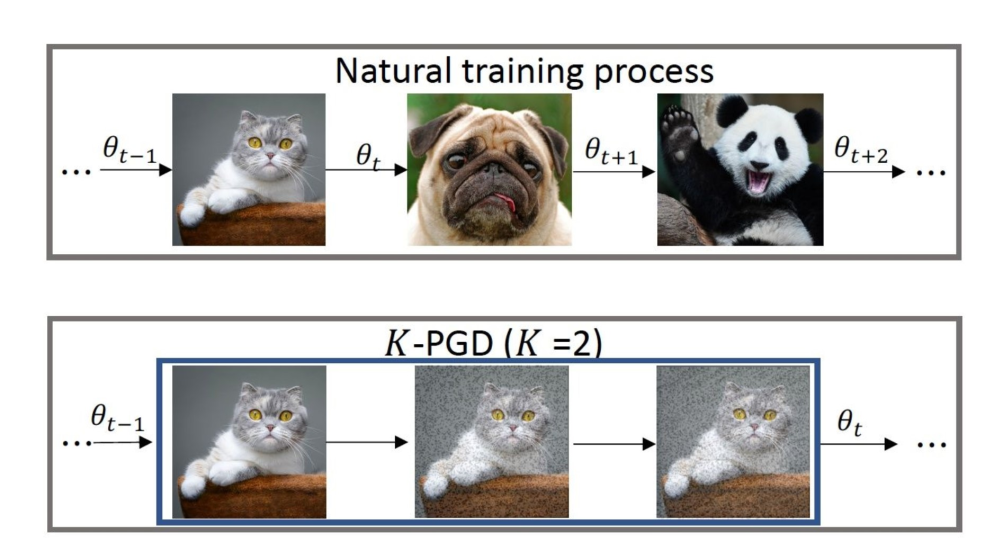
\includegraphics[width=0.8\textwidth]{figure/adv_train.png}
    \caption{在传统的训练过程中加入对抗训练}
    \label{fig:adv_train}
\end{figure}

\section{常见攻击手段}
对于深度学习模型特别是图像相关的神经网络模型提出了许多种类的扰动攻击:FGSM、
I-FGSM、雅克比矩阵攻击、单像素攻击、DeepFool 等等 \cite{DBLP:conf/iclr/LiuCLS17} \cite{DBLP:conf/iclr/KurakinGB17}。
\begin{figure}[htbp]
    \centering
    \includegraphics[width=0.8\textwidth]{figure/attack_rep.pdf}
    \caption{不同攻击手段的成本和效果}
    \label{fig:attack_rep}
\end{figure}

如图\ref{fig:attack_rep}所示,其中FGSM为扰动攻击领域最经典的基于梯度的基础攻击。雅可比攻击为
增加了二阶近似的攻击,单像素攻击和DeepFool为人工精心构造的攻击,k-FGSM为FGSM多步迭代的版本。
这其中,FGSM和由之衍生出的Step-LL等攻击常用于对抗训练。

\section{黑盒/白盒攻击}
将生成扰动的模型成为源模型,扰动攻击的对象称为目标模型。根据源模型和目标模型是否
一致,将攻击划分为黑盒和白盒两种\cite{DBLP:journals/corr/abs-1810-00069}。具体示意如图\ref{fig:black_white}所示。
\begin{figure}[htbp]
    \centering
    \includegraphics[width=0.8\textwidth]{figure/transfer.pdf}
    \caption{黑盒攻击与白盒攻击}
    \label{fig:black_white}
\end{figure}

在白盒攻击中,攻击者对于当前模型具有全部的知识,他可以给定任意输入,根据模型的中间结果和最终输出计算出理想的
攻击,从而成功hack模型;在黑盒攻击中,攻击者仅知道对于某些特定的输入,模型产生的最终输出,无法通过计算
产生理想的攻击。在这种情况下,攻击者通过寻找一个已知的中介(proxy)模型,在该模型上产生扰动攻击,再转移到
需要hack的模型上。

\section{扰动攻击的可转移性}
\begin{figure}[htbp]
    \centering
    \includegraphics[width=0.8\textwidth]{figure/transfer_prop.pdf}
    \caption{黑盒攻击与白盒攻击}
    \label{fig:transfer_prop}
\end{figure}
深度学习模型中的扰动攻击具有可转移性的特点。具体如图\ref{fig:transfer_prop}所示,对于一个Unknow Network
进行黑盒攻击时,找到一个完成相似任务的网络模型Proxy,基于该网络产生扰动攻击,再转移到Unknow Network上。
实验表明,这样的攻击有较高的可能性取得成功。

\begin{table}[htbp]
    \centering
    \begin{tabular}{ccccccc}
               & RMSD & ResNet-152 & ResNet-101 & ResNet-50 & VGG-16 & GoogleNet \\ \hline
    ResNet-152 & 22.8 & 0\%        & 13\%       & 18\%      & 19\%   & 11\%      \\
    ResNet-101 & 23.8 & 19\%       & 0\%        & 21\%      & 21\%   & 12\%      \\
    ResNet-50  & 22.9 & 23\%       & 20\%       & 0\%       & 21\%   & 18\%      \\
    VGG-16     & 22.5 & 22\%       & 17\%       & 17\%      & 0\%    & 5\%       \\
    GoogleNet  & 22.6 & 39\%       & 38\%       & 34\%      & 19\%   & 0\%       \\ \hline
    \end{tabular}
    \caption{扰动攻击在不同模型间的转移\cite{DBLP:conf/iclr/LiuCLS17}}
    \label{tab:attack_transfer}
\end{table}

具体实验结果如表\ref{tab:attack_transfer}所示,其中ResNet、VGG-16、GoogleNet为不同的神经网络模型,表格的第(i, j)
个单元格为模型i上产生的扰动攻击作用在模型j上时的攻击失败率。对角线上均为白盒攻击,因此攻击失败率为0。实验结果表明,在其他模型
上产生的扰动攻击可以以较大的成功率转移到其他模型上并成功攻击目标模型。
